\begin{figure*}
  \centering
  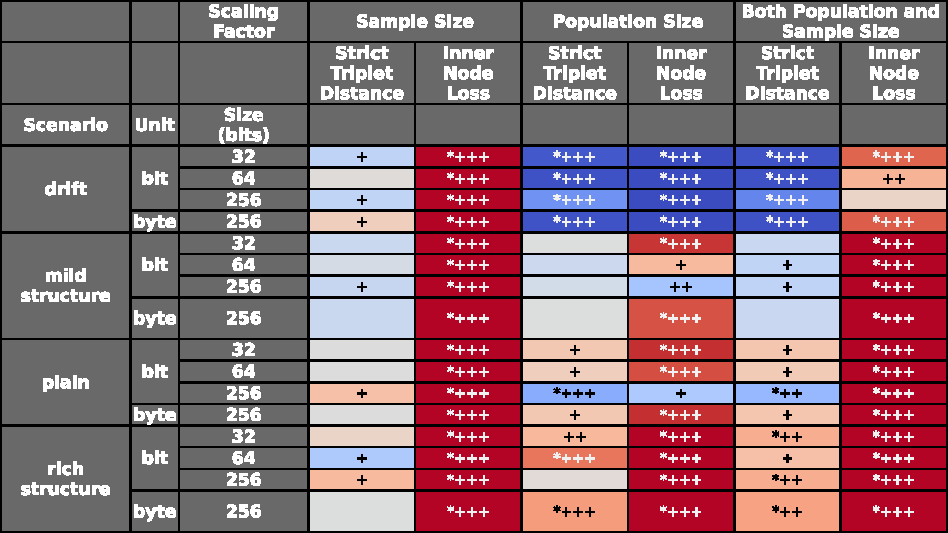
\includegraphics[width=\textwidth]{binder/binder/dsamp-popsize-scale/outplots/dsamp-popsize-scale-steady.pdf}
  \caption{%
   \textbf{Comparison of reconstruction quality between small and large downsample and population sizes under steady retention policy.}
   \footnotesize
    First column considers sample size in isolation, second column considers scaling population size in isolation, and third column considers scaling population and sample size together.
    Color coding reflects non-parametric comparison between reconstruction quality measure values, with red indicating degraded reconstruction quality at larger scale and blue indicating improved reconstruction quality at larger scale.
    Larger downsample size is 8,000 taxa and smaller downsample size is 500 taxa.
    Larger population size is 65,536 and smaller population size is 4,096.
    Experiments used steady retention policy with column-based implementation.
    In cell annotations, +'s indicate small, medium, and large effect sizes using the Cliff's delta statistic and *'s indicate statistical significance at $\alpha = 0.05$ via Mann-Whitney U test.
  }
  \label{fig:dsamp-popsize-scale-steady}
\end{figure*}
